\documentclass[english]{article}
\usepackage[a4paper, total={6in, 8in}]{geometry}
\usepackage{graphicx}
\title{Capstone Project - The Battle of Neighborhoods \\ Wine Bars and Shops in Paris}
\author{Tom Hohweiller, PhD.}
\date{}
\begin{document}	
	\maketitle
	% SSSSSSSSSSSSSSSSSSSSSSSSSSSSSSSSSSSSSSSSSSS %
	\section{Introduction}
	In the business of restaurants, Paris has a big competition. Being one of the most visited cities in the world, the french capital is one of the best places to eat in France. That's why, when looking for an area to establish one's wine bar (or shop), the decision must come with great reflection. A restaurant owner in another city in France came to ask me which area in Paris would make a wine bar successful. My client was mostly preoccupied with the density of restaurants and existing wine bars and shops (which in Paris is quite high). So to have a great location, a study must be done to find. After discussion, we came to an agreement that looking for an \textit{arrondissement} (a subdivision of French cities) that have already a good number of restaurants is a must: the logic being that not a lot of person would go out in an area with few restaurants or wine bars. Finally, my client is also underlining the fact that having a wine bar in an area with only shops will damage his benefits (people won't come at dinner time). So, we'll look for a populated area (within an \textit{arrondissement}) where restaurants are present.
	% SSSSSSSSSSSSSSSSSSSSSSSSSSSSSSSSSSSSSSSSSSS %
	\section{Methodology}
	Our methodology to tackle this problem is quite straightforward since the business question was quite clear. From this very clear idea, the buisiness understanding was quite fast. In order to satify this client, four steps can emerged:
	\begin{itemize}
		\item[1.] Extract every venues in each \textit{arrondissement} to have a better view of the business situation
		\item[2.] Study the number of restaurants as well as the number per 1000 residents (for wine bars or shops also)
		\item[3.] After selecting a \textit{arrondissement}, refine the venues and clustering them to identify small area with proeminent restaurants
		\item[4.] Finally, choosing the best area will be our best location in Paris
	\end{itemize}
	From these four bullet points, the next steps can be defined.
	% SsSsSsSsSsSsSsSsSsSsSsSsSsSsSsSsSsSsSsSsSsS %
	\subsection{Data}
	% SssSssSssSsssSsssSsssSsssSssssSsssSsssSsssSsssSssSsSsSsSsSsSsSsSsS %
	\subsubsection{Data requirements}
	The first problem to address would be what data to gather. The list would be
	\begin{itemize}
		\item Coordinates of each \textit{arrondissement} of Paris ($20$ of them) and their population
		\item Venues in Paris for each \textit{arrondissement}. Scanning large and removing duplicates to ensure that all venues are gathered only once. With these information
		\begin{itemize}
			\item Name of the venue
			\item Coordinates
			\item Venue category
			\item Postal code (for sorting later on to refine the model)
		\end{itemize}
	\end{itemize}
	% SssSssSssSsssSsssSsssSsssSssssSsssSsssSsssSsssSssSsSsSsSsSsSsSsSsS %
	\subsubsection{Data collection}
	Two types of information are presents, two types of information canal will be used. For the coordinate and population, (french) Wikipedia web page has a section for population and coordinate for each \textit{arrondissement} with the same format as described here:
	%fffffffffffffffffffffffffffffffffffffffffffffffffffffffffffffffffffffff%
	\begin{figure}[h]
		\centering
		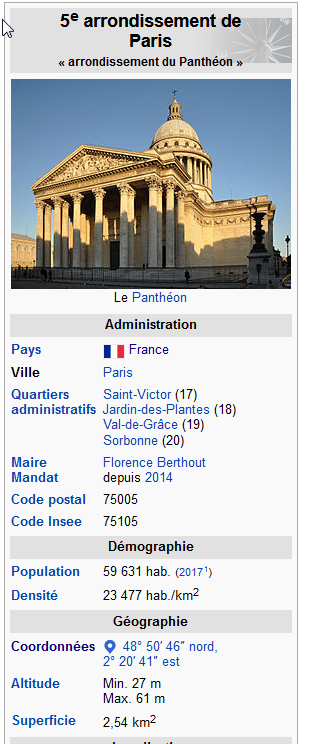
\includegraphics[width=0.25\linewidth,keepaspectratio]{Figures/Exemple_Arrondissement_Wikipedia}
		\caption{Example of the wikipedia webpage for the fifth \textit{arrondissement}.}
		\label{Arrondissement}
	\end{figure}
	%fffffffffffffffffffffffffffffffffffffffffffffffffffffffffffffffffffffff%
	Luckily enough, all have the same URL format as followed: $https://fr.wikipedia.org/wiki/\boldmath{X}\_arrondissement\_de\_Paris$ where $X$ is the be replaced with:
	\begin{equation}
		X = \{1er, 2e, 3e, 4e, 5e, 6e, 7e, 8e, 9e, 10e, 11e, 12e, 13e, 14e, 15e, 16e, 17e, 18e, 19e, 20e\}
	\end{equation}
	
	Finally, for the venues data, Foursquare API gave us the perfect tool. With regular calls, the name of the venues, coordinates, and venue categories can be gather using the coordinate of each \textit{arrondissement}. Then, premium calls can be made to have postal codes of each venue selected within an \textit{arrondissement}.
	% SssSssSssSsssSsssSsssSsssSssssSsssSsssSsssSsssSssSsSsSsSsSsSsSsSsS %
	\subsubsection{Data understanding}
	Collected population and \textit{arondissement} data will be correct since the population was updated in the last five years (and coordinates are... coordinates). However, one can expect a relatively low number of restaurants and wine bars or shops. This would be easily explained since Foursquare is not an overly used venue's rating platform. But since the use of the Foursquare API is accessible and the number of venues on the website is representative of the real number of venues (in a few orders). One can assume that for this study, of the relation between the number of restaurants and the population, the extracted dataset is big enough.	
	% SssSssSssSsssSsssSsssSsssSssssSsssSsssSsssSsssSssSsSsSsSsSsSsSsSsS %
	\subsubsection{Data preparation}
	In this study, four data sets are easily extracted from the previous steps:
	\begin{itemize}
		\item[1-] DataSet of each \textit{arrondissement}, with its:
		\begin{itemize}
			\item Name
			\item Coordinates
			\item Population
		\end{itemize}
		\item[2-] DataSet of all the venues (for each \textit{arrondissement}), with:
		\begin{itemize}
			\item Coordinates
			\item Venue name
			\item Venue category
			\item Venue Id
		\end{itemize}
		\item[3-] DataSet for restaurants and wine bars and shops, with:
		\begin{itemize}
			\item Total number of restaurants for each \textit{arrondissement}
			\item Total number of wine bars and shops for each \textit{arrondissement}
			\item Total number of restaurants per 1000 residents for each \textit{arrondissement}
			\item Total number of wine bars and shops per 1000 residents for each \textit{arrondissement}
		\end{itemize}
		\item[4-] DataSet for the selected \textit{arrondissement}, with:
		\begin{itemize}
			\item Venue name 
			\item Venue coordinates
			\item Venue category (all type of venues)
			\item Venue Id
			\item Venue postal code
		\end{itemize}
	\end{itemize}
	% SSSSSSSSSSSSSSSSSSSSSSSSSSSSSSSSSSSSSSSSSSS %
	\section{Modeling}
	As said before, this study can be split into four ways:
	\begin{itemize}
		\item[1.] Extract every venues in each \textit{arrondissement} to have a better view of the business situation
		\item[2.] Study the number of restaurants as well as the number per 1000 residents (for wine bars or shops also)
		\item[3.] After selecting a \textit{arrondissement}, refine the venues and clustering them to identify small area with proeminent restaurants
		\item[4.] Finally, choosing the best area will be our best location in Paris
	\end{itemize}
	Firstly, this work will be done using Python for its several packages available to us that will make every part of the former plan quick. Moreover, it does not require high computational requirements. For these reasons, Python is a very good option.
	% SssSssSssSsssSsssSsssSsssSssssSsssSsssSsssSsssSssSsSsSsSsSsSsSsSsS %
	\subsubsection{Webscrapping}
	As said previously, coordinates and population about each \textit{arrondissement} will be done using webscrapping techniques. Using \texttt{requests} and \texttt{beautifulsoup} packages, one can request a html page and look for the table (presented Figure.\ref{Arrondissement}). After getting latitude, longitude and population for each \textit{arrondissement}, a dataframe will be created using \texttt{pandas}. For the following fields: ['Arr','Latitude'\\,'Longitude','Population'].	
	% SssSssSssSsssSsssSsssSsssSssssSsssSsssSsssSsssSssSsSsSsSsSsSsSsSsS %
	\subsubsection{Venues}
	After having all coordinates and population, it's time to get all the venues per \textit{arrondissement}. To do so, Foursquare will be used thanks to their API. Sending a request with \texttt{latitude}, \texttt{longitude} and a \texttt{radius}. It returns a JSON file that contains all kinds of information. In this study, the ones that will be saved are:
	\begin{itemize}
		\item Coordinates
		\item Venue name
		\item Venue category
		\item Venue Id
	\end{itemize}
	To get all the venues, the \texttt{radius} to $2000$ meters, which is way big enough to get all relevant venues. But, since the information is getting through looping over the \textit{arrondissement}, venues can appear multiples times. Dropping duplicates can be easily done using \texttt{pandas} (function \texttt{drop.duplicates()}), also creating a data frame containing all informations about venues in Paris. With the following fields:	
	\begin{itemize}
		\item Coordinates
		\item Venue name
		\item Venue category
		\item Venue Id
	\end{itemize}
	% SssSssSssSsssSsssSsssSsssSssssSsssSsssSsssSsssSssSsSsSsSsSsSsSsSsS %
	\subsubsection{Restaurants and wine bars/shops}
	Previously gathered venues information are about all categories. So, will retain (for the study's sake) only venues category that contains \textit{Restaurant} or \textit{wine}. From this informations, using \texttt{pandas} functions, calculating the number of restaurants and wine bars and shops in an \textit{arrondissement} is easy. Moreover, thanks to the population gather during the first stage of data collection, the computation of the number of restaurants and wine bars, and shops per $1000$ residents are quickly done. From this information, plotting the total number of restaurants and wine-related venues can be done. Using, the number of venues per $1000$ residents will be the criteria to pick an \textit{arrondissement} to continue our study.
	% SssSssSssSsssSsssSsssSsssSssssSsssSsssSsssSsssSssSsSsSsSsSsSsSsSsS %
	\subsubsection{Best \textit{arrondissement}}
	Finding the correct \textit{arrondissement} won't cut it. It can be rather small, our even area with restaurants can be between several \textit{arrondissement}. So, the model needs to be refined. Let's call $N$ the best \textit{arrondissement}. First of all, venues need to be sorted. Venues outside the $N$ \textit{arrondissement} will be discarded, but to be thorough, the ones that border $N$ will also be considered. This can be easily done by looking at the postal code. Send a request to the Foursquare API for the venues listed the $N$ \textit{arrondissement} (which gather a lot of them since the radius was very large), will return postal code (premium call using venues Id, gathered before). A map can be plotted using the \texttt{folium} package with selected venues. At this point, a certain number of clusters will be identified visually (let's note it $n_c$). Using the \textit{k-means} algorithm, an area will be created, from which a top $5$ venues category can be extracted. From these $n_c$ clusters of venues, selected ones with similar venues will be easily done.
	% SSSSSSSSSSSSSSSSSSSSSSSSSSSSSSSSSSSSSSSSSSS %
	\section{Evaluation}
	Three evaluations are to be done in this study:
	\begin{itemize}
		\item The best \textit{arrondissement}: $N$
		\item Which \textit{arrondissement} to pick around $N$
		\item Number of cluster to defined: $n_c$
	\end{itemize}
	$N$ will be defined by looking at the overall results of the number of restaurants. Picking $N$ as the upper $50\%$ of \textit{arrondissement} would be ideal. \textit{Arrondissement} around $N$ can be done using any type of maps (google maps for example), which is rather quick. Finally, $n_c$ will be chosen using the map created by \texttt{folium}.
	% SSSSSSSSSSSSSSSSSSSSSSSSSSSSSSSSSSSSSSSSSSS %
	\section{Results and discussion}
	% SssSssSssSsssSsssSsssSsssSssssSsssSsssSsssSsssSssSsSsSsSsSsSsSsSsS %
	\subsection{Webscrapping and venues gathering}
	Using \texttt{beautifulsoup} and the Foursquare API, dataframes representing each \textit{arrondissement} and their venues are created as showed below.	
	%fffffffffffffffffffffffffffffffffffffffffffffffffffffffffffffffffffffff%
	\begin{figure}[h]
		\centering
		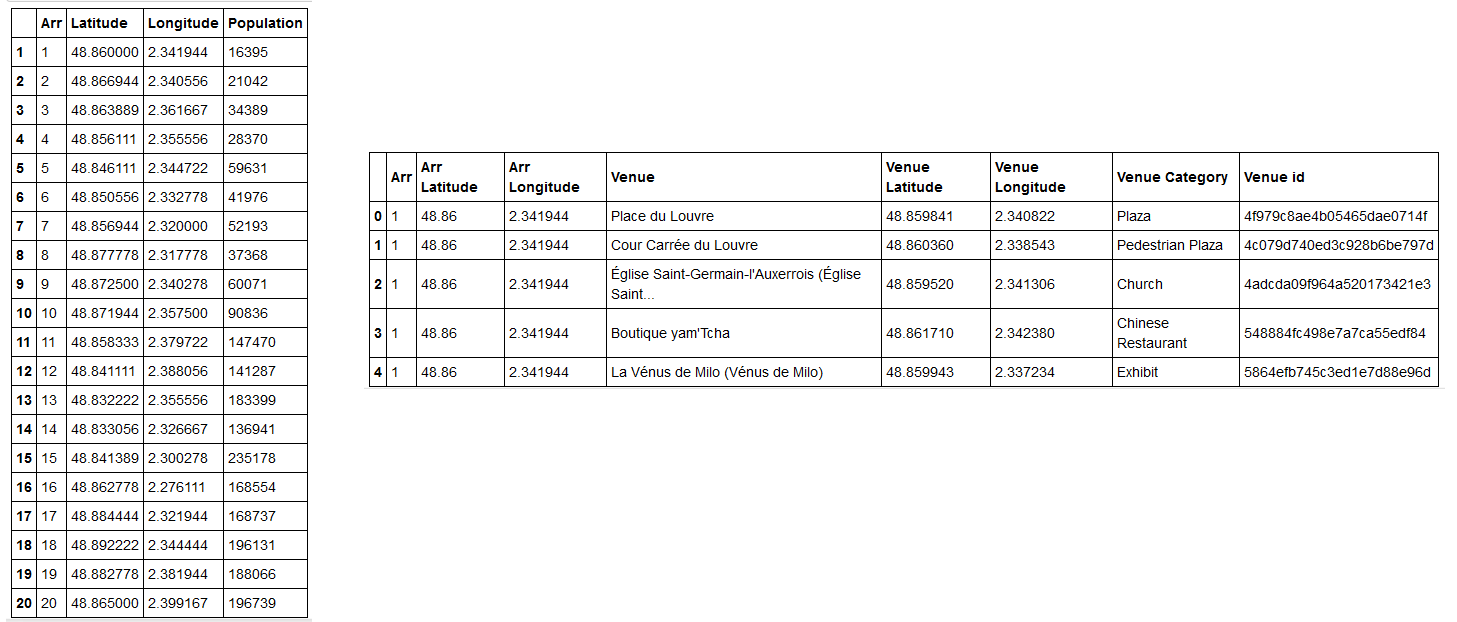
\includegraphics[width=\linewidth,keepaspectratio]{Figures/DataFrameArrVenues}
		\caption{Dataframe of each \textit{arrondissement} (left) and data frame of each venues (right).}
		\label{DataFrames}
	\end{figure}
	%fffffffffffffffffffffffffffffffffffffffffffffffffffffffffffffffffffffff%	
	% SssSssSssSsssSsssSsssSsssSssssSsssSsssSsssSsssSssSsSsSsSsSsSsSsSsS %
	\subsubsection{Restaurants and wine bars/shops}
	From the venues containing only \textit{Restaurant} or \textit{wine}, and calculating the total number of each one and the ratio (with $1000$ residents). The following bar plots can be plotted:
	%fffffffffffffffffffffffffffffffffffffffffffffffffffffffffffffffffffffff%
	\begin{figure}[h]
		\centering
		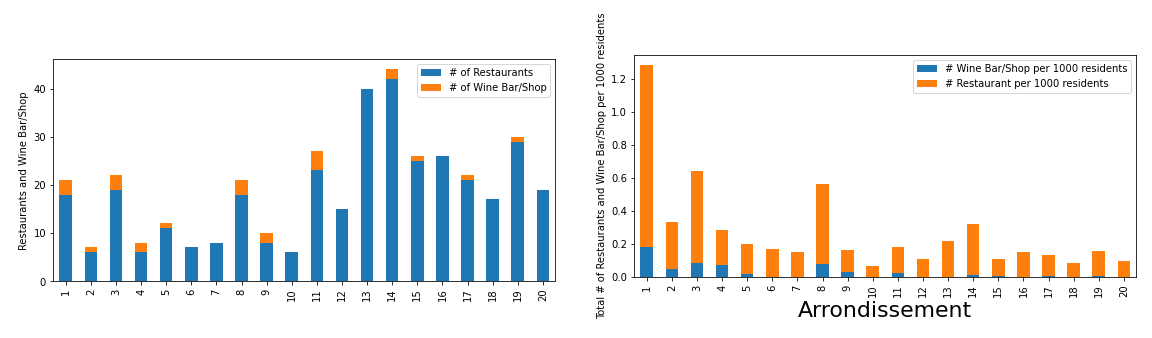
\includegraphics[width=\linewidth,keepaspectratio]{Figures/BarPlots}
		\caption{Bar plots of the total number of restaurants and wine bars/shops (left). Number of restaurants and wine bars/shops per $1000$ residents (right).}
		\label{BarPlots}
	\end{figure}
	%fffffffffffffffffffffffffffffffffffffffffffffffffffffffffffffffffffffff%	
	From these plots (Figure.\ref{BarPlots}), the third \textit{arrondissement} will be chosen, it is in the mean values, over the $50\%$ threshold set before. Moreover, geographically, it is quite centered in Paris, then:
	\begin{equation}
		N = 3
	\end{equation}
	% SssSssSssSsssSsssSsssSsssSssssSsssSsssSsssSsssSssSsSsSsSsSsSsSsSsS %
	\subsection{Best \textit{arrondissement}}
	In this particular results, the following \textit{arrondissement} will be kept: $1$st, $2$nd, $3$rd, $4$th, $10$th and $11$th (all of them being around the $3$rd). Extracting postal codes, the following dataframe is created:
	%fffffffffffffffffffffffffffffffffffffffffffffffffffffffffffffffffffffff%
	\begin{figure}[h]
		\centering
		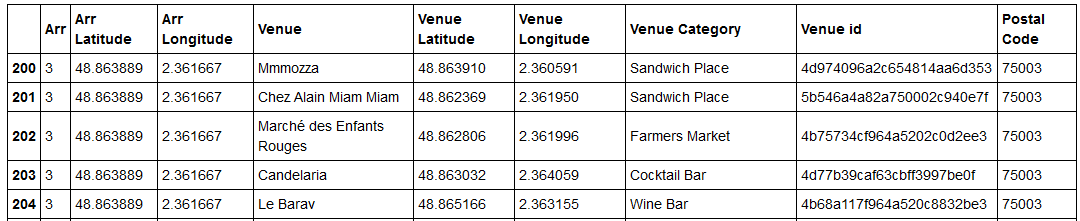
\includegraphics[width=\linewidth,keepaspectratio]{Figures/DataFraleThird}
		\caption{Dataframe of the third \textit{arrondissement} with additional information.}
		\label{DataFramesThird}
	\end{figure}
	%fffffffffffffffffffffffffffffffffffffffffffffffffffffffffffffffffffffff%	
	From this point, looking at the spatial repartition of the venues can help decide the value of $n_c$ (the number of clusters). So, the following \texttt{folium} map is generated:
	%fffffffffffffffffffffffffffffffffffffffffffffffffffffffffffffffffffffff%
	\begin{figure}[h!]
		\centering
		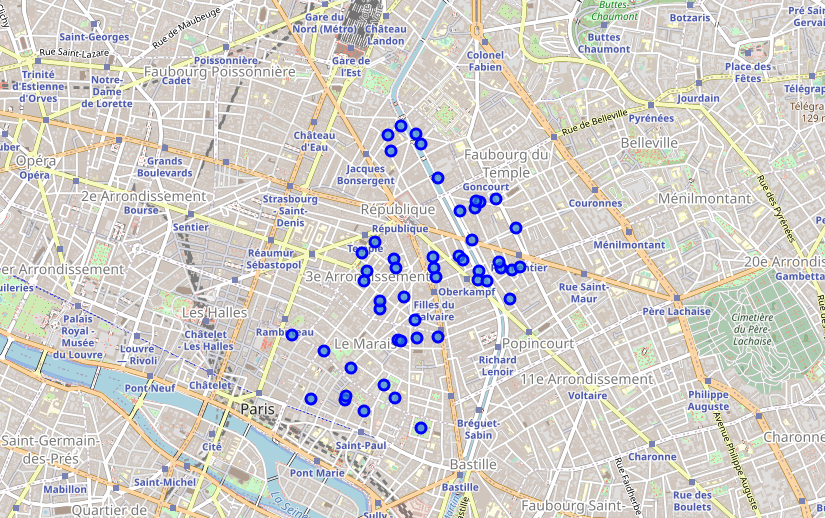
\includegraphics[width=0.60\linewidth,keepaspectratio]{Figures/FoliumUnclustered}
		\caption{Spatial repartition of the venues of the third \texttt{arrondissement} and around.}
		\label{FoliumMap}
	\end{figure}
	%fffffffffffffffffffffffffffffffffffffffffffffffffffffffffffffffffffffff%	
	At this point, visually the number of four clusters can be selected ($n_c = 4$). Using the \textit{k-means} algorithm, and the previous map, the area can be color-coded as follow:
	%fffffffffffffffffffffffffffffffffffffffffffffffffffffffffffffffffffffff%
	\begin{figure}[h!]
		\centering
		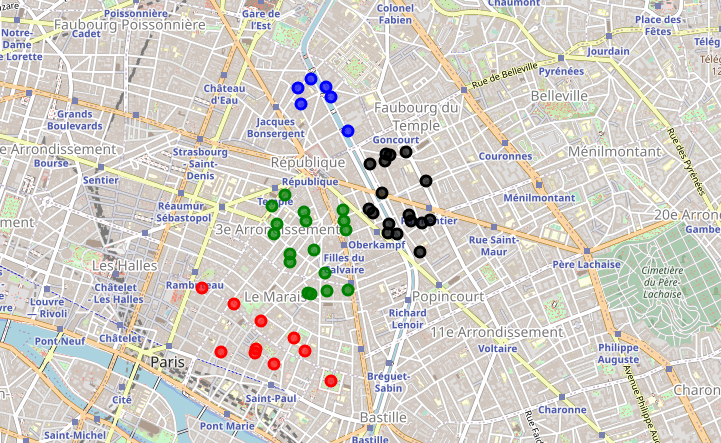
\includegraphics[width=0.60\linewidth,keepaspectratio]{Figures/FoliumClustered}
		\caption{Spatial repartition of the venues of the third \texttt{arrondissement} and around - color coded with respect with cluster label.}
		\label{FoliumMapColored}
	\end{figure}
	%fffffffffffffffffffffffffffffffffffffffffffffffffffffffffffffffffffffff%
	From each cluster, the top $5$ venue can be extracted, generating the following table:	
	%fffffffffffffffffffffffffffffffffffffffffffffffffffffffffffffffffffffff%
	\begin{figure}[h!]
		\centering
		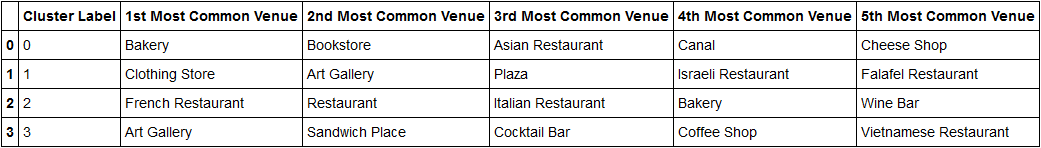
\includegraphics[width=\linewidth,keepaspectratio]{Figures/TopFive}
		\caption{Top $5$ venues category for each clusters.}
		\label{ClustersVenueCat}
	\end{figure}
	%fffffffffffffffffffffffffffffffffffffffffffffffffffffffffffffffffffffff%
	Finally, the cluster label $2$ gives an area with existing restaurants (that the other have more day-related activities: shops, gallery, ...). Finally, from this study the best area to be for a wine bar/shop will be around the following circle:
	%fffffffffffffffffffffffffffffffffffffffffffffffffffffffffffffffffffffff%
	\begin{figure}[h]
		\centering
		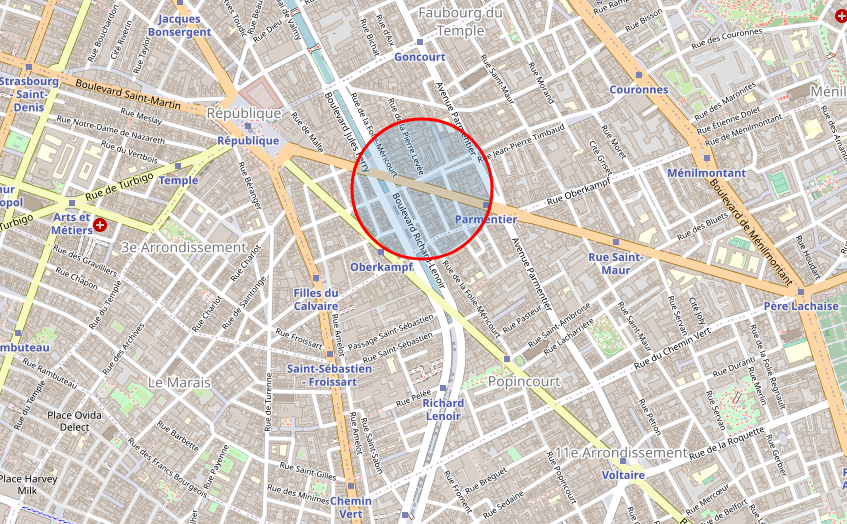
\includegraphics[width=0.60\linewidth,keepaspectratio]{Figures/FoliumFinal}
		\caption{Best location for a wine bar/shop in Paris.}
		\label{FinalLocation}
	\end{figure}
	%fffffffffffffffffffffffffffffffffffffffffffffffffffffffffffffffffffffff%		
	% SSSSSSSSSSSSSSSSSSSSSSSSSSSSSSSSSSSSSSSSSSS %
	\section{Conclusion}	
	This study aims at defining the best location for a particular venue in Paris. Looking for the best place to have a wine bar/shop in this city was done using web scrapping to get information about each subdivision of Paris. Getting the venue's information with Foursquare was rapidly done giving all the information needed. The \textit{arrondissement} with the best number of restaurants (and per $1000$ residents) was the third one (already existing venues but not too many). Considering all surrounded \textit{arrondissement} gave a map of all venues around this point. Looking at spatial clusters, the best location was picked by looking at the top $5$ venues category. Fitting the type of venue the clients wants to open, just east of the Republic place was chosen.
\end{document}